\hypertarget{nublogger_8h}{
\section{/Users/nikki/nublabs/nub.datalogger/hardware/temperature\_\-sensor\_\-Terciopelo/nublogger.h File Reference}
\label{nublogger_8h}\index{/Users/nikki/nublabs/nub.datalogger/hardware/temperature\_\-sensor\_\-Terciopelo/nublogger.h@{/Users/nikki/nublabs/nub.datalogger/hardware/temperature\_\-sensor\_\-Terciopelo/nublogger.h}}
}
{\tt \#include $<$HardwareSerial.h$>$}\par
{\tt \#include $<$string.h$>$}\par
{\tt \#include \char`\"{}communications.h\char`\"{}}\par


Include dependency graph for nublogger.h:\nopagebreak
\begin{figure}[H]
\begin{center}
\leavevmode
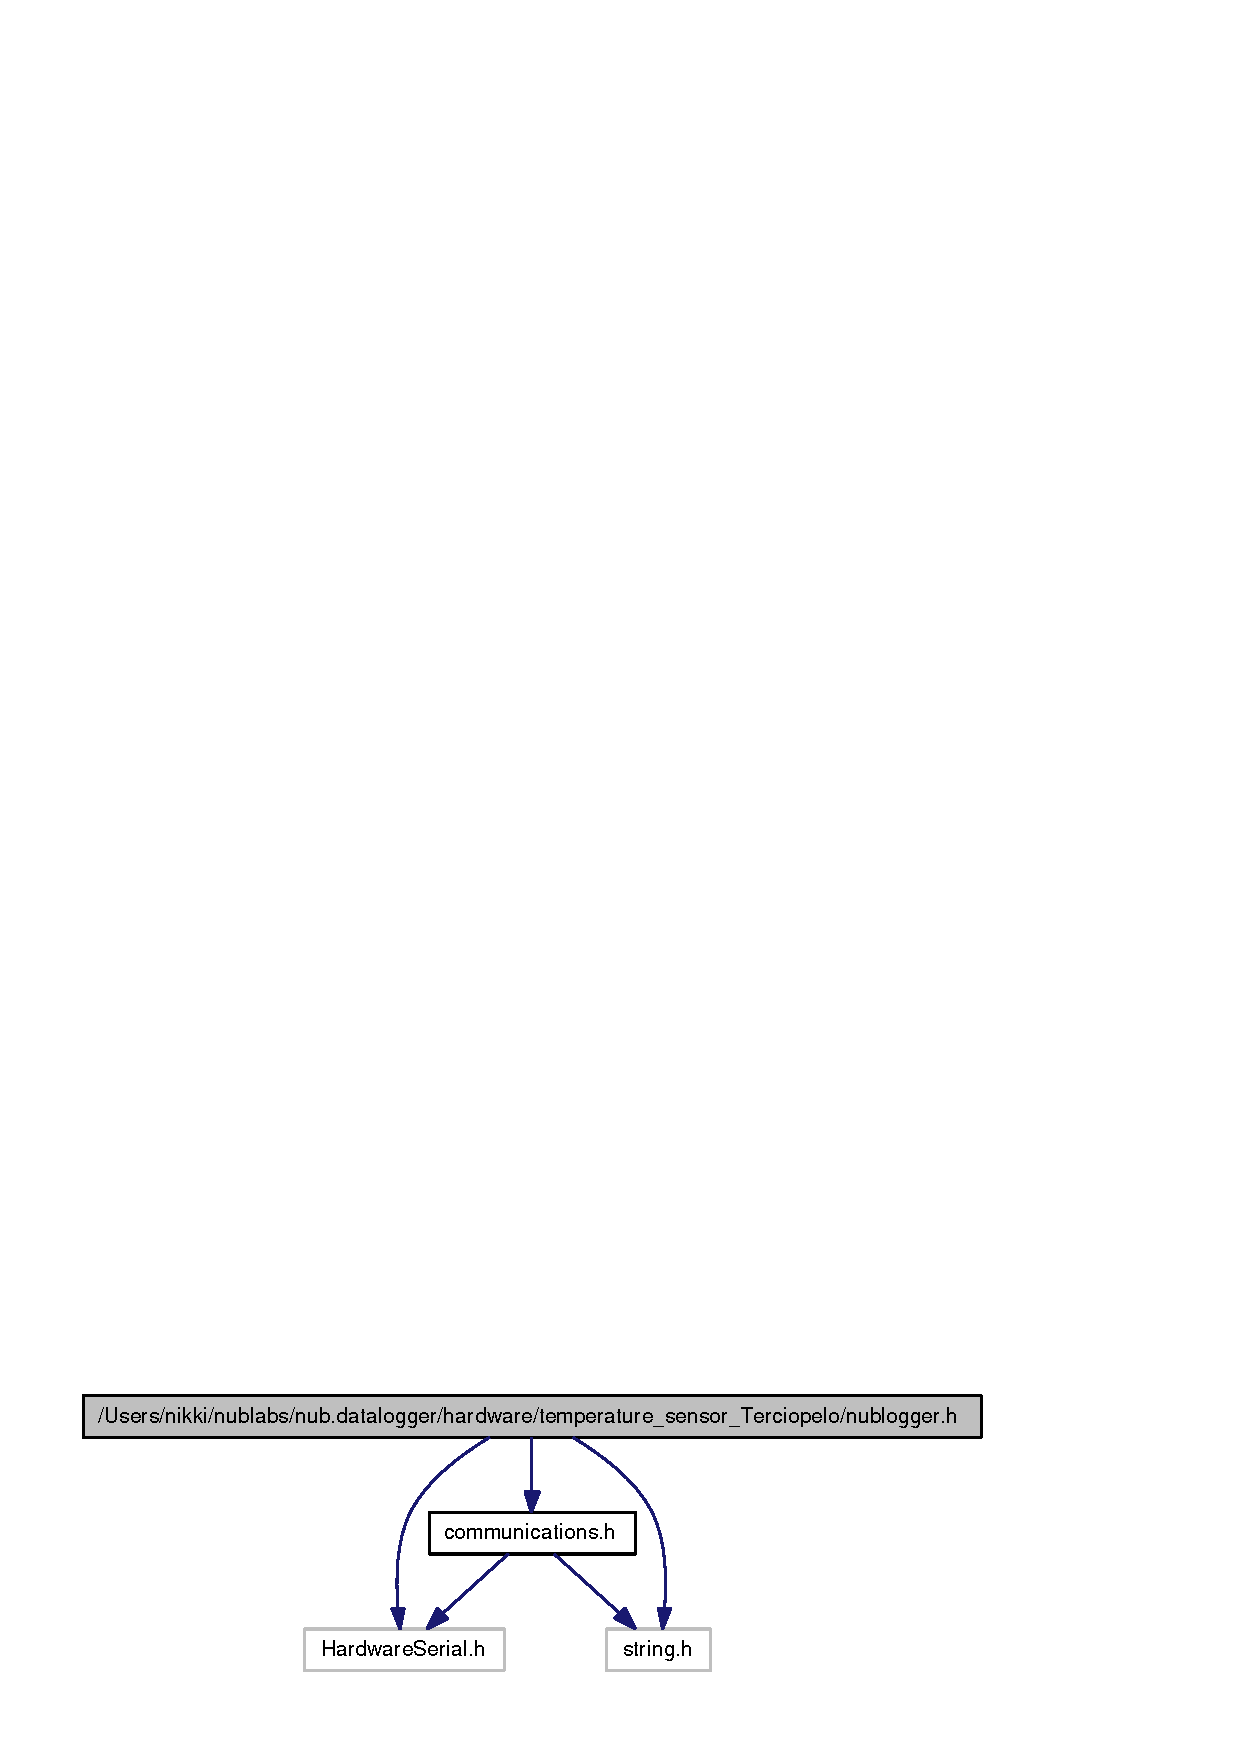
\includegraphics[width=237pt]{nublogger_8h__incl}
\end{center}
\end{figure}
\subsection*{Functions}
\begin{CompactItemize}
\item 
void \hyperlink{nublogger_8h_e369b3765489ee8bd0ea791c1843630f}{configure} ()
\begin{CompactList}\small\item\em \hyperlink{applet_2nublogger_8h_e369b3765489ee8bd0ea791c1843630f}{configure()} runs if the computer is trying to change the sensor's sample rate \item\end{CompactList}\item 
void \hyperlink{nublogger_8h_3fdb2350c3f98c0de0f0ae3c831a8b14}{discover} ()
\begin{CompactList}\small\item\em This function tells the computer of the datalogger's existence. \item\end{CompactList}\end{CompactItemize}


\subsection{Function Documentation}
\hypertarget{nublogger_8h_e369b3765489ee8bd0ea791c1843630f}{
\index{nublogger.h@{nublogger.h}!configure@{configure}}
\index{configure@{configure}!nublogger.h@{nublogger.h}}
\subsubsection[{configure}]{\setlength{\rightskip}{0pt plus 5cm}void configure ()}}
\label{nublogger_8h_e369b3765489ee8bd0ea791c1843630f}


\hyperlink{applet_2nublogger_8h_e369b3765489ee8bd0ea791c1843630f}{configure()} runs if the computer is trying to change the sensor's sample rate 

In \hyperlink{applet_2nublogger_8h_e369b3765489ee8bd0ea791c1843630f}{configure()}, the datalogger sends a LISTENING message to the computer, indicating that it's ready to receive data. The computer sends three ints: the hours, minutes and seconds of the sample interval, followed by a checksum byte that's the sum of the ints modulo 256. The sensor computes a checksum on the received data. If its checksum matches, it sends an ACKNOWLEDGE message back to the computer and updates its sample interval information. If the checksum does not match, it sends a CHECKSUM\_\-ERROR\_\-PLEASE\_\-RESEND message, asking the computer to send the three ints again, followed by a checksum. If the sensor can't get a valid message (with a matching checksum) after three tries, it gives up, sends a CHECKSUM\_\-ERROR\_\-GIVING\_\-UP message to the computer and keeps its original sample interval information 

Definition at line 15 of file nublogger.h.

\begin{Code}\begin{verbatim}16 { 
17 }
\end{verbatim}
\end{Code}


\hypertarget{nublogger_8h_3fdb2350c3f98c0de0f0ae3c831a8b14}{
\index{nublogger.h@{nublogger.h}!discover@{discover}}
\index{discover@{discover}!nublogger.h@{nublogger.h}}
\subsubsection[{discover}]{\setlength{\rightskip}{0pt plus 5cm}void discover ()}}
\label{nublogger_8h_3fdb2350c3f98c0de0f0ae3c831a8b14}


This function tells the computer of the datalogger's existence. 

When the sensor turns on, it runs \hyperlink{applet_2nublogger_8h_3fdb2350c3f98c0de0f0ae3c831a8b14}{discover()}. It sends a MESSAGE\_\-START message, a DISCOVER\_\-ME message, and its name out to the computer and waits for acknowledgement. The computer can send back a plain \char`\"{}ACKNOWLEDGE\char`\"{} message, which means that the sensor should run using its default configuration values. The computer can also send back an \char`\"{}ACKNOWLEDGE\_\-AND\_\-CONFIGURE\char`\"{} message, which means that it has configuration data for the sensor. If the sensor gets this message, it'll run \hyperlink{applet_2nublogger_8h_e369b3765489ee8bd0ea791c1843630f}{configure()} to receive the data from the computer. 

Definition at line 27 of file nublogger.h.

References ACKNOWLEDGE, ACKNOWLEDGE\_\-AND\_\-CONFIGURE, configure(), DISCOVER\_\-ME, discovered, getByte(), MESSAGE\_\-END, MESSAGE\_\-START, name, and TRUE.

\begin{Code}\begin{verbatim}28 { 
29   unsigned char checksum=0;
30   int i=0;
31   Serial.print(MESSAGE_START, BYTE);
32   Serial.print(DISCOVER_ME,BYTE);
33   Serial.print(name);
34   while(name[i]!=0)
35   {
36     checksum+=name[i];
37     i++;
38   }
39   checksum+=DISCOVER_ME;
40   Serial.print(checksum,BYTE);
41   Serial.print(MESSAGE_END,BYTE);
42 
43   int receivedByte=getByte(100);     //looks for a byte on the serial port with a 100ms timeout
44   if(receivedByte==ACKNOWLEDGE)
45     discovered=TRUE;
46   if(receivedByte==ACKNOWLEDGE_AND_CONFIGURE)
47     {
48       discovered=TRUE;
49       configure();
50     }
51   
52 }
\end{verbatim}
\end{Code}


